\documentclass[border={7pt 0pt 7pt 0pt},varwidth]{standalone}
\usepackage{amsmath}
\usepackage[dvipsnames]{xcolor}%colors
\usepackage{tikz-cd,tikz-3dplot} 
\usepackage{diagbox}
\usepackage{makecell}
\usepackage{adjustbox}
\usepackage{multirow}
\usepackage[width=0.5,tiewidth=0.7]{strands}
\usepackage{array}

\newcommand{\fakestar}{*}
\begin{document}

\begin{table}[]
\[
\begin{array}{ccc}
   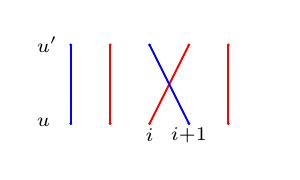
\begin{tikzpicture}
    \node at (-0.3,0.06) {$\scriptstyle u\phantom{'}$};
    \node at (2.3,0.06) {$\phantom{\scriptstyle u'}$};
    \node at (-0.3,1) {$\scriptstyle u'$};
    \node at (1,-0.15) {$\scriptstyle i$};
    \node at (1.5,-0.15) {$\scriptstyle i+1$};
    \tie[color=blue,bull=1,bulletie=0.01,style=solid]{{1,1},{1,0}}
    \tie[color=red,bull=1,bulletie=0.01,style=solid]{{2,1},{2,0}}
    \tie[color=red,bull=1,bulletie=0.01,style=solid]{{4,1},{3,0}}
    \tie[color=blue,bull=1,bulletie=0.01,style=solid]{{3,1},{4,0}}
    \tie[color=red,bull=1,bulletie=0.01,style=solid]{{5,1},{5,0}} 
    \end{tikzpicture}        &   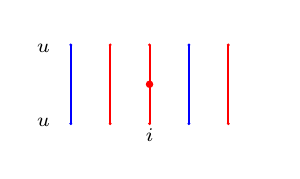
\begin{tikzpicture}
      \node at (-0.3,0.06) {$\scriptstyle u\phantom{'}$};
      \node at (2.3,0.06) {$\phantom{\scriptstyle u'}$};
      \node at (-0.3,1) {$\scriptstyle u\phantom{'}$};
      \node at (1,-0.15) {$\scriptstyle i$};
      \tie[color=blue,bull=1,bulletie=0.01,style=solid]{{1,1},{1,0}}
      \tie[color=red,bull=1,bulletie=0.01,style=solid]{{2,1},{2,0}}
      \tie[color=red,bull=1,bulletie=0.01,style=solid]{{3,1},{3,0}}
      \tie[color=blue,bull=1,bulletie=0.01,style=solid]{{4,1},{4,0}}
      \tie[color=red,bull=1,bulletie=0.01,style=solid]{{5,1},{5,0}} 
      \tie{3}
      \end{tikzpicture}       &   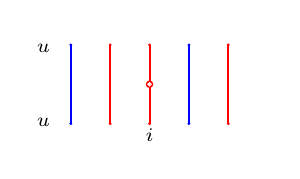
\begin{tikzpicture}
         \node at (-0.3,0.06) {$\scriptstyle u\phantom{'}$};
         \node at (2.3,0.06) {$\phantom{\scriptstyle u'}$};
         \node at (-0.3,1) {$\scriptstyle u\phantom{'}$};
         \node at (1,-0.15) {$\scriptstyle i$};
         \tie[color=blue,bull=1,bulletie=0.01,style=solid]{{1,1},{1,0}}
         \tie[color=red,bull=1,bulletie=0.01,style=solid]{{2,1},{2,0}}
         \tie[color=red,bull=1,bulletie=0.01,style=solid]{{3,1},{3,0}}
         \tie[color=blue,bull=1,bulletie=0.01,style=solid]{{4,1},{4,0}}
         \tie[color=red,bull=1,bulletie=0.01,style=solid]{{5,1},{5,0}} 
         \tie{3}\tie[color=white,bulletie=0.02]{3}
         \end{tikzpicture}         \\
D_i^{u,u'} & e_i^{u} & (e_i^{u})^{-1}\!
\end{array}
\]
\end{table}
\end{document}